\documentclass[tikz,border=14pt]{standalone}
\usepackage{tikz}
\usetikzlibrary{positioning, arrows.meta, calc, backgrounds}

\definecolor{ctrlFill}{RGB}{255,224,189}
\definecolor{ctrlBrd}{RGB}{204,120,30}
\definecolor{compFill}{RGB}{255,252,204}
\definecolor{compBrd}{RGB}{180,160,40}
\definecolor{locFill}{RGB}{210,235,210}
\definecolor{locBrd}{RGB}{90,150,90}
\definecolor{gloFill}{RGB}{210,225,245}
\definecolor{gloBrd}{RGB}{80,110,180}
\definecolor{gmFill}{RGB}{245,210,210}
\definecolor{gmBrd}{RGB}{180,80,80}
\definecolor{keyBg}{RGB}{245,245,245}
\definecolor{enRed}{RGB}{190,0,0}

\tikzset{
  every node/.style={font=\ttfamily\small},
  B/.style={draw, rounded corners=1pt, inner sep=4pt, align=center, minimum height=0.65cm},
  CTRL/.style={B, fill=ctrlFill, draw=ctrlBrd},
  COMP/.style={B, fill=compFill, draw=compBrd},
  LOC/.style={B,  fill=locFill,  draw=locBrd},
  GLO/.style={B,  fill=gloFill,  draw=gloBrd},
  GM/.style={B,   fill=gmFill,   draw=gmBrd},
  AR/.style={-{Stealth[length=5pt]}, thick, black},
  RD/.style={-{Stealth[length=5pt]}, thick, enRed},
  TH/.style={black, thin},
}

%% Layout: pipeline centered at x=260; thread area split at x=260
%% Left column cx=130, right column cx=390
%% Each thread structure has LSU | ALU | PC with visible spacing between boxes.
%% Upper row y=228, upper Reg y=268, lower row y=306, lower Reg y=346

\begin{document}
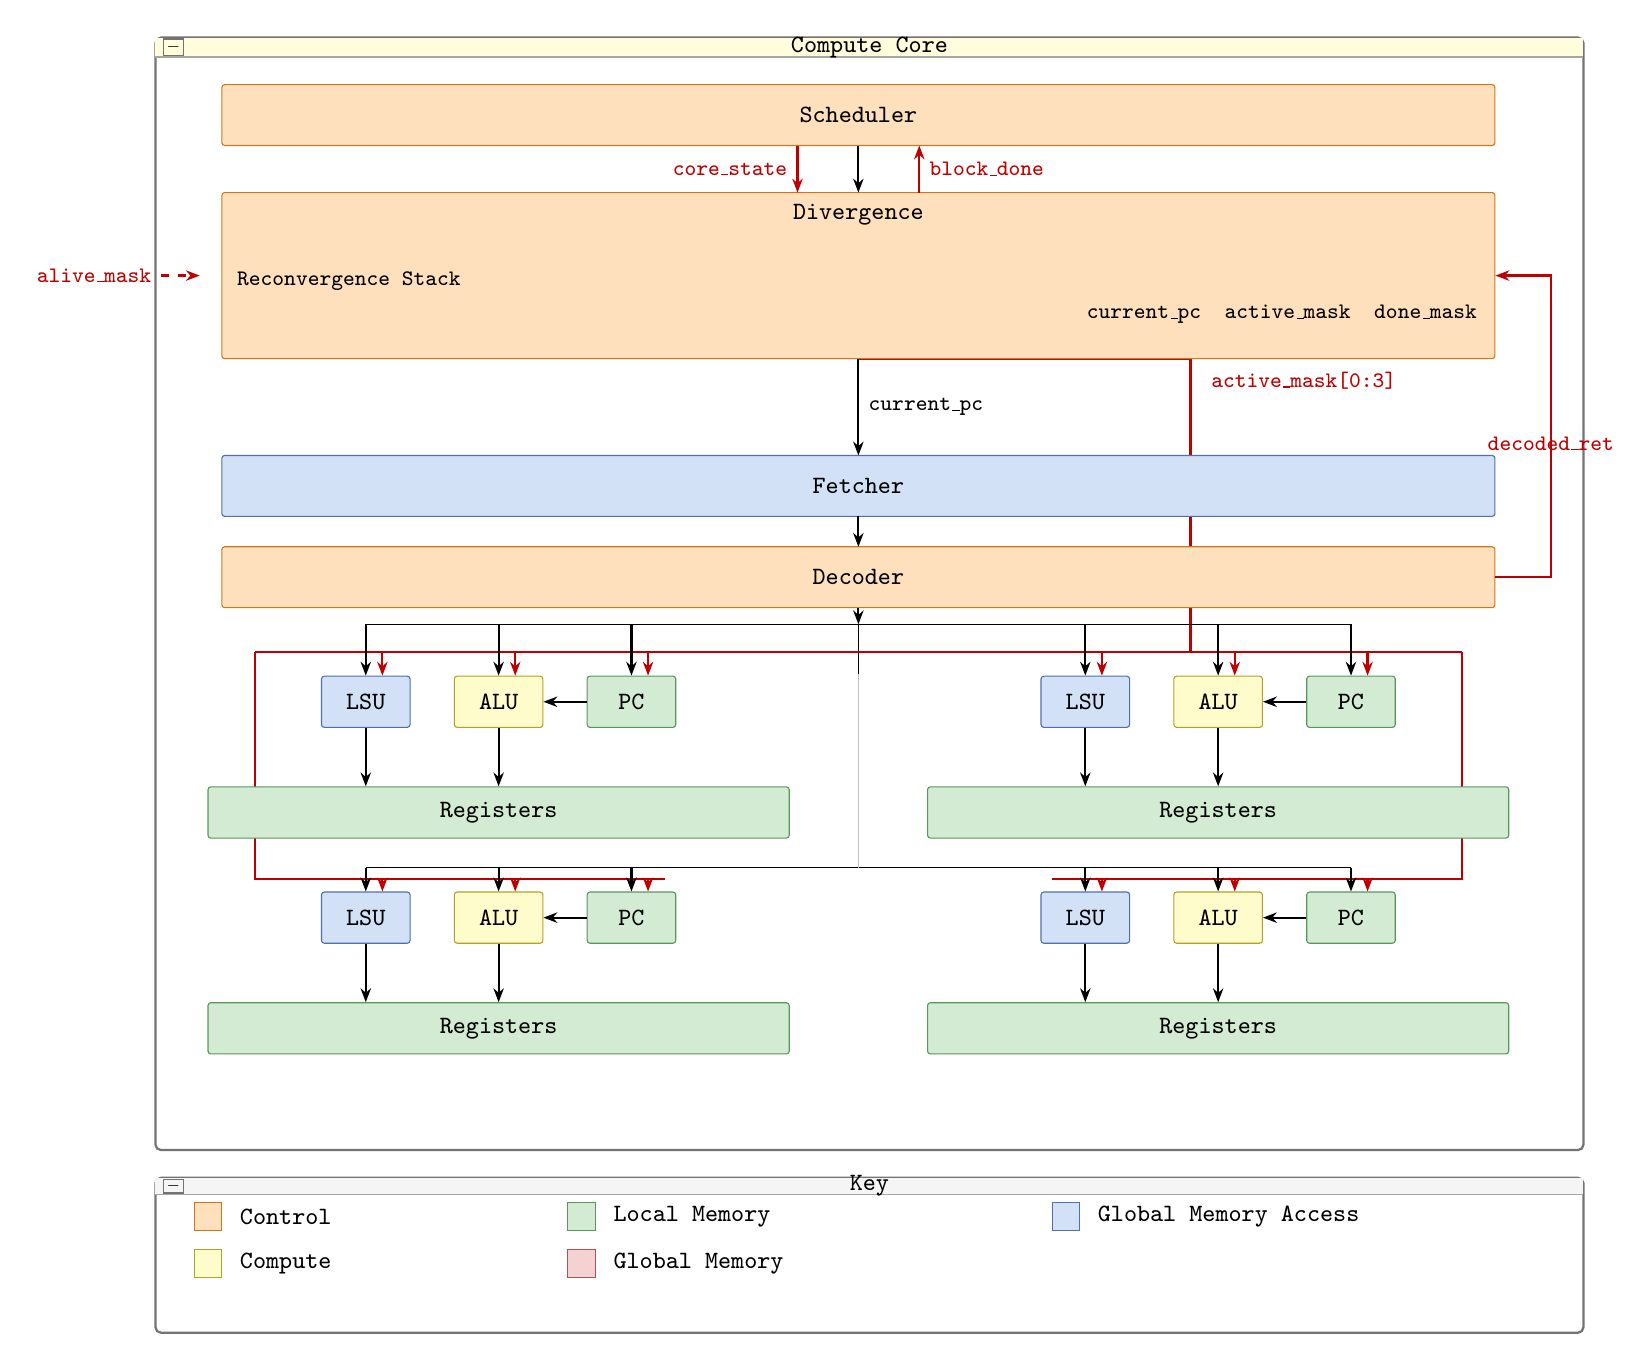
\begin{tikzpicture}[x=1pt, y=1pt, yscale=-1]

%% ═══════════════════════════════════════════════════════════════════════════
%%  PART A — pipeline
%% ═══════════════════════════════════════════════════════════════════════════

\node[CTRL, minimum width=460pt, minimum height=22pt] (SCH) at (260,16) {\textbf{Scheduler}};
\node[CTRL, minimum width=460pt, minimum height=60pt] (DIV) at (260,74) {};
\node[font=\ttfamily\small\bfseries] at (260,52) {Divergence};
\node[font=\ttfamily\footnotesize, anchor=west] at (32,76) {Reconvergence Stack};
\node[font=\ttfamily\footnotesize, anchor=east] at (487,88)
  {current\_pc \enspace active\_mask \enspace done\_mask};
\node[GLO, minimum width=460pt, minimum height=22pt] (FET) at (260,150) {\textbf{Fetcher}};
\node[CTRL,minimum width=460pt, minimum height=22pt] (DEC) at (260,183) {\textbf{Decoder}};

\draw[AR] (260,27)  -- (260,44);
\draw[RD] (238,27)  -- node[left,font=\ttfamily\footnotesize,enRed]{core\_state}(238,44);
\draw[RD] (282,44)  -- node[right,font=\ttfamily\footnotesize,enRed]{block\_done}(282,27);
\draw[AR] (260,104) -- node[right,font=\ttfamily\footnotesize]{current\_pc}(260,139);
\draw[AR] (260,161) -- (260,172);

\draw[RD,dashed] (8,74) -- (22,74);
\node[font=\ttfamily\footnotesize,enRed,anchor=east] at (8,74) {alive\_mask};

\draw[RD] (DEC.east) -- ++(20,0) |- (DIV.east)
  node[near start,below,font=\ttfamily\footnotesize,enRed]{decoded\_ret};

%% ═══════════════════════════════════════════════════════════════════════════
%%  Decoder fan-out bus (splits to left / right columns)
%% ═══════════════════════════════════════════════════════════════════════════
\def\busY{200}
\def\maskY{210}
\def\lowerBusY{288}
\def\sW{32pt}
\def\rW{210pt}
\def\yU{228}
\def\yRu{268}
\def\yL{306}
\def\yRl{346}

\draw[AR] (260,194) -- (260,\busY);
\draw[TH] (82,\busY) -- (438,\busY);

%% Lower-row decoder routes come down the center divider, then branch outward
%% to the lower-left and lower-right structures.
\draw[TH] (260,\busY) -- (260,\lowerBusY);
\draw[TH] (260,\lowerBusY) -- (82,\lowerBusY);
\draw[TH] (260,\lowerBusY) -- (438,\lowerBusY);

%% active_mask enable bus
\draw[enRed,thick] (42,\maskY) -- (478,\maskY);
\begin{scope}[on background layer]
  \draw[enRed,thick] (260,104) -- ++(120,0) |- (475,\maskY);
\end{scope}
\node[font=\ttfamily\footnotesize,enRed,anchor=west] at (384,112) {active\_mask[0:3]};

%% Lower-row enable routes are separated from the black decoder routes.
\draw[enRed,thick] (42,\maskY) -- (42,292) -- (190,292);
\draw[enRed,thick] (478,\maskY) -- (478,292) -- (330,292);

%% Center column divider (left | right)
\draw[black!25,thin] (260,218) -- (260,\lowerBusY);

%% ═══════════════════════════════════════════════════════════════════════════
%%  Macro-like: one structure (LSU|ALU|PC + Registers), identical all four
%%  #1 prefix  #2 cx  #3 y row  #4 y reg
%% ═══════════════════════════════════════════════════════════════════════════

%% --- Left column, upper (T0) cx=130 ---
\node[GLO,minimum width=\sW] (LU_L) at (82,\yU) {LSU};
\node[COMP,minimum width=\sW] (LU_A) at (130,\yU) {ALU};
\node[LOC,minimum width=\sW] (LU_P) at (178,\yU) {PC};
\draw[AR] (LU_P.west) -- (LU_A.east);

\node[LOC,minimum width=\rW] (LU_R) at (130,\yRu) {Registers};
\draw[AR] (LU_L.south) -- (LU_L.south |- LU_R.north);
\draw[AR] (LU_A.south) -- (LU_A.south |- LU_R.north);

\draw[AR] (82,\busY) -- (LU_L.north);
\draw[AR] (130,\busY) -- (LU_A.north);
\draw[AR] (178,\busY) -- (LU_P.north);

\draw[RD] (88,\maskY) -- ([xshift=6pt]LU_L.north);
\draw[RD] (136,\maskY) -- ([xshift=6pt]LU_A.north);
\draw[RD] (184,\maskY) -- ([xshift=6pt]LU_P.north);

%% --- Left column, lower (T1) ---
\node[GLO,minimum width=\sW] (LL_L) at (82,\yL) {LSU};
\node[COMP,minimum width=\sW] (LL_A) at (130,\yL) {ALU};
\node[LOC,minimum width=\sW] (LL_P) at (178,\yL) {PC};
\draw[AR] (LL_P.west) -- (LL_A.east);

\node[LOC,minimum width=\rW] (LL_R) at (130,\yRl) {Registers};
\draw[AR] (LL_L.south) -- (LL_L.south |- LL_R.north);
\draw[AR] (LL_A.south) -- (LL_A.south |- LL_R.north);

\draw[AR] (82,\lowerBusY) -- (LL_L.north);
\draw[AR] (130,\lowerBusY) -- (LL_A.north);
\draw[AR] (178,\lowerBusY) -- (LL_P.north);

\draw[RD] (88,292) -- ([xshift=6pt]LL_L.north);
\draw[RD] (136,292) -- ([xshift=6pt]LL_A.north);
\draw[RD] (184,292) -- ([xshift=6pt]LL_P.north);

%% --- Right column, upper (T2) cx=390 ---
\node[GLO,minimum width=\sW] (RU_L) at (342,\yU) {LSU};
\node[COMP,minimum width=\sW] (RU_A) at (390,\yU) {ALU};
\node[LOC,minimum width=\sW] (RU_P) at (438,\yU) {PC};
\draw[AR] (RU_P.west) -- (RU_A.east);

\node[LOC,minimum width=\rW] (RU_R) at (390,\yRu) {Registers};
\draw[AR] (RU_L.south) -- (RU_L.south |- RU_R.north);
\draw[AR] (RU_A.south) -- (RU_A.south |- RU_R.north);

\draw[AR] (342,\busY) -- (RU_L.north);
\draw[AR] (390,\busY) -- (RU_A.north);
\draw[AR] (438,\busY) -- (RU_P.north);

\draw[RD] (348,\maskY) -- ([xshift=6pt]RU_L.north);
\draw[RD] (396,\maskY) -- ([xshift=6pt]RU_A.north);
\draw[RD] (444,\maskY) -- ([xshift=6pt]RU_P.north);

%% --- Right column, lower (T3) ---
\node[GLO,minimum width=\sW] (RL_L) at (342,\yL) {LSU};
\node[COMP,minimum width=\sW] (RL_A) at (390,\yL) {ALU};
\node[LOC,minimum width=\sW] (RL_P) at (438,\yL) {PC};
\draw[AR] (RL_P.west) -- (RL_A.east);

\node[LOC,minimum width=\rW] (RL_R) at (390,\yRl) {Registers};
\draw[AR] (RL_L.south) -- (RL_L.south |- RL_R.north);
\draw[AR] (RL_A.south) -- (RL_A.south |- RL_R.north);

\draw[AR] (342,\lowerBusY) -- (RL_L.north);
\draw[AR] (390,\lowerBusY) -- (RL_A.north);
\draw[AR] (438,\lowerBusY) -- (RL_P.north);

\draw[RD] (348,292) -- ([xshift=6pt]RL_L.north);
\draw[RD] (396,292) -- ([xshift=6pt]RL_A.north);
\draw[RD] (444,292) -- ([xshift=6pt]RL_P.north);

%% Outer panels
\begin{scope}[on background layer]
  \draw[black!55,thick,rounded corners=2pt] (6,-12) rectangle (522,390);
  \fill[compFill!70] (6,-12) rectangle (522,-5);
  \draw[black!35] (6,-5)--(522,-5);
\end{scope}
\node[font=\ttfamily\small\bfseries] at (264,-8.5) {Compute Core};
\draw[black!55] (9,-11.5) rectangle (16,-5.5);
\node[font=\ttfamily\tiny] at (12.5,-8.5) {$-$};

\begin{scope}[on background layer]
  \draw[black!55,thick,rounded corners=2pt] (6,400) rectangle (522,456);
  \fill[keyBg] (6,400) rectangle (522,406);
  \draw[black!35] (6,406)--(522,406);
\end{scope}
\node[font=\ttfamily\small] at (264,403) {Key};
\draw[black!55] (9,400.5) rectangle (16,405.5);
\node[font=\ttfamily\tiny] at (12.5,403) {$-$};

\fill[ctrlFill](20,409) rectangle(30,419); \draw[ctrlBrd](20,409) rectangle(30,419);
\node[anchor=west,font=\ttfamily\small] at (33,414) {Control};
\fill[locFill] (155,409) rectangle(165,419); \draw[locBrd](155,409) rectangle(165,419);
\node[anchor=west,font=\ttfamily\small] at (168,414) {Local Memory};
\fill[gloFill] (330,409) rectangle(340,419); \draw[gloBrd](330,409) rectangle(340,419);
\node[anchor=west,font=\ttfamily\small] at (343,414) {Global Memory Access};
\fill[compFill](20,426) rectangle(30,436); \draw[compBrd](20,426) rectangle(30,436);
\node[anchor=west,font=\ttfamily\small] at (33,431) {Compute};
\fill[gmFill]  (155,426) rectangle(165,436); \draw[gmBrd](155,426) rectangle(165,436);
\node[anchor=west,font=\ttfamily\small] at (168,431) {Global Memory};

\end{tikzpicture}
\end{document}
